\documentclass[10pt,foldmark,notumble]{leaflet}
\renewcommand*\foldmarkrule{.3mm}
\renewcommand*\foldmarklength{5mm}
\usepackage{float} %Bilder einbinden
\usepackage[utf8]{inputenc} %Umlaute
\usepackage{graphicx} %Graphiken
\usepackage{hyperref} %wg URL
\usepackage{amsmath}
\usepackage[T1]{fontenc}
\usepackage{textcomp}
\usepackage{mathptmx}
\usepackage{microtype}%Blocksatz
\usepackage[scaled=0.9]{helvet}

\usepackage[T1]{fontenc}
\newcommand{\changefont}[3]{
\fontfamily{#1} \fontseries{#2} \fontshape{#3} \selectfont} %http://www.math.tu-dresden.de/~rudl/latex/fonts.pdf


\makeatletter
\def\ptmTeX{T\kern-.1667em\lower.5ex\hbox{E}\kern-.075emX\@}
\DeclareRobustCommand{\ptmLaTeX}{L\kern-.3em
{\setbox0\hbox{T}%
%\vb@xt@ % :-)
\vbox to\ht0{\hbox{%
\csname S@\f@size\endcsname
\fontsize\sf@size\z@
\math@fontsfalse\selectfont
A}%
\vss}%
}%
\kern-.12em
\ptmTeX}
\makeatother
\let\TeX=\ptmTeX
\let\LaTeX=\ptmLaTeX
\usepackage{shortvrb}
\MakeShortVerb{\|}
\usepackage{url}
\usepackage[dvipsnames,usenames]{color}
\definecolor{LIGHTGRAY}{gray}{.9}
\newcommand\Lpack[1]{\textsf{#1}}
\newcommand\Lclass[1]{\textsf{#1}}
\newcommand\Lopt[1]{\texttt{#1}}
\newcommand\Lprog[1]{\textit{#1}}

\newcommand*\defaultmarker{\textsuperscript\textasteriskcentered}

\CutLine*{1}% Dotted line without scissors
%\CutLine{6}% Dotted line with scissors
\CutLine*{6}% 

%%%%%%%%%%%%%%%%%%%%%%%%%%%%%%%%%%%%%%%%%%%%%%%%%%%%%%%%%%%%%%%%%%%%%
\usepackage{Sweave}
\begin{document}
\Sconcordance{concordance:Flyer_Lisa_V012.tex:Flyer_Lisa_V012.Rnw:%
1 53 1 1 0 208 1}


\vfill
\section{Energetische Gesichts- \& Körperstraffung}
Die Access Energetic Facelift® Anwendung ist eine wundervolle Verwöhn- und Verjüngungsmöglichkeit für das Gesicht und den ganzen Körper.
%\vfill
\section{Ayurvedische Gesichtsmassage}
Massage mit warmen Öl.
%\vfill
\section{Energiearbeit mit Atlantischer Lichtheilung}
Bei dieser Methode wird durch das Auflegen der Hände Energie übertragen. Entspannung und Wohlbefinden stellen sich ein. Ihre Selbstheilkräfte werden angeregt. 
%\vfill
\section{Ganzheitliche Kopfschmerzmassage}
Bei stress- und spannungsbedingten Kopfsschmerzen. 
Kopfschmerzen, Migräne und Nackenverspannungen sind weit verbreitet. Mit der Headache Massage biete ich eine ganz spezielle Massage - Technik, die Ihnen Linderung verschaffen kann. Diese Massage bringt Ihnen mehr Lebensqualität, Entspannung und Wohlbefinden. 
\vfill


\newpage
%%%%%%%%%%%%%%%%%%%%%%%%%%%%%%%%%%%%%%%%%%%%%%%%%%%%%%%%%%%%%%%%%%%%%
%\vspace*{20mm}

\vfill
\section{Rückenmassage}
Eine besondere Technik aus der Kopfschmerzmassage zur Entspannung. 
\vfill
\section{Metamorphose Behandlung}
Metamorphose ist eine sanfte Lichtarbeit an den Füßen, Händen und Kopf. Der Begriff "Metamorphose" heißt wörtlich übersetzt "Umwandlung". Dies bezieht sich auf Lebensmuster, die umgewandelt werden. So wie die Raupe zum Schmetterling wird, entfaltet sich hier das angelegte Potential des Menschen.\\
\\
Die Metamorphose ist vom Ansatz her bewusstseins\-erweiternd und wirkt lösend auf negative seelische Strukturen und Lebensmuster, die sich in der pränatalen (vorgeburtlichen) Phase gebildet haben.
\vfill
\section{Nieren gut, alles gut - Ingwerkompresse}
Dient der Öffnung und Entgiftung der Nieren und damit einer Stabilisierung der Nierentätigkeit. 2-3 malige Auflage des Wickels und Ruhezeit. 
%\vfill
\section{Klopfmassage zur Erdung}
Hier biete ich Ihnen die Möglichkeit nach kurzer Zeit ihren Körper zu energetisieren, Spannungen zu lösen und sich geerdet und lebendig zu fühlen. 
%\begin{itemize}
%\item Straffung der Falten und Gesichtslinien
%\item Straffung der Gesichtsmuskeln sowie der ganzen Haut
%\item verbesserte Sehkraft
%\item schnellerer Heilungsprozess von Narbengewebe
%\item strahlendere, gesündere Haut
%\end{itemize}
%\vfill
%\section{}
\begin{figure}[h] %[b]
\begin{center}
 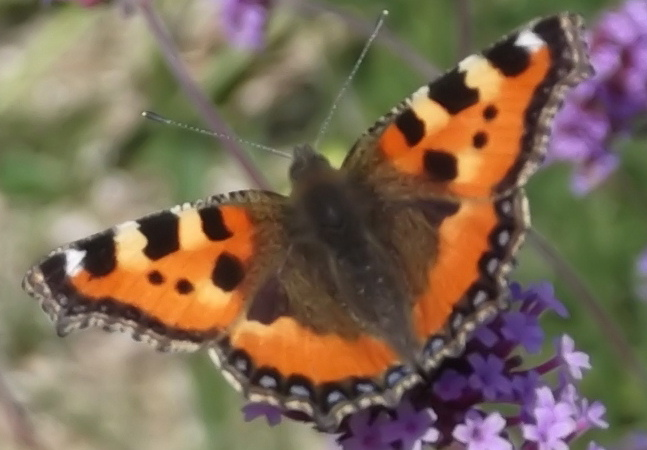
\includegraphics [scale=.25]{Schmetterling3.JPG}
 %\caption{Dies ist die Bildunterschrift}
 %\label{figure}
 \end{center}
 \end{figure}
\newpage
%%%%%%%%%%%%%%%%%%%%%%%%%%%%%%%%%%%%%%%%%%%%%%%%%%%%%%%%%%%%%%%%%%%%%
%\vspace*{20mm}


%%%%%%%%%%%%%%%%%%%%%%%%%%%%%%%%%%%%%%%%%%%%%%%%%%%%%%%%%%%%%%%%%%%%%
%\vspace*{20mm}
\section{Meine Sitzungen und Preise}
%\centerline  {\bf {Meine Sitzungen und Preise}}%{\large}
\begin{tabular}{p{65mm}cr}%\hline\hline %
Bars Sitzung (Blockaden lösen durch Berührung von 32 Punkten am Kopf)  &    \\
(ca 45-60 Minuten) &    40,-€  \\
\\
\hline
\\
Facelifting  &    \\
(ca. 60 Minuten) &    50,-€\\
\\
\hline
\\
Körperlifting   &   \\
(ca. 60 Minuten) &    50,-€\\
\\
\hline
\\
Face- und Körperlifting   &    \\
(ca. 90 Minuten) &    80,-€\\
\\
\hline
\\
Gesichtsmassage nach Ayurveda &    \\
(ca. 30 Minuten) &    25,-€ \\
\\
\hline 
\\
Atlantische Lichtheilung für Mensch und Tier  &    \\
(ca. 60 Minuten) &    40,-€ \\
\\
\hline
\\
Ganzheitliche Kopfschmerzmassage &     \\
(ca. 60 Minuten) &    50,-€ \\
\\
\hline
\\
Rückenmassage &    \\
(ca. 40 Minuten) &    30,-€ \\
\\
\hline
\\
Metamorphose Massage  &     \\
(ca. 60 - 75 Minuten) &    50,-€ \\
\\
\hline
\\
Klopfmassage zur Erdung  &    \\
(ca. 20 Minuten) &    15,-€ \\
\\
\hline
\\
Ingwerkompresse  &     \\
(ca. 45 Minuten) &    25,-€ \\

\end{tabular}

%%%%%%%%%%%%%%%%%%%%%%%%%%%%%%%%%%%%%%%%%%%%%%%%%%%%%%%%%%%%%%%%%%%%%
\newpage
\vfill
%\vspace*{20mm}
\begin{figure}[h]
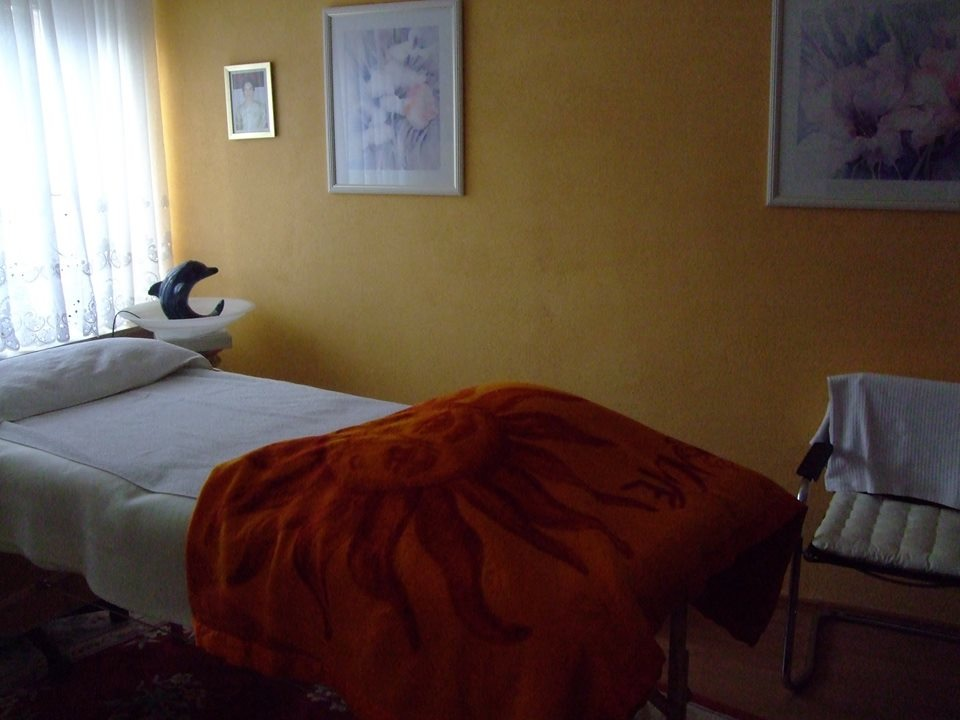
\includegraphics [scale=.25]{Bild1.jpg}
\caption{Das Behandlungszimmer}
%\label{figure}
 \end{figure}


\section{ }
\centerline {\LARGE {\bf {Ich freue mich auf Ihren Besuch!}}}


\section{ }
Meine Anwendungen dienen der Entspannung und regen die Selbstheilungskräfte an. Sie ersetzten nicht den Arzt oder den Heilpraktier. 
\vfill

%%%%%%%%%%%%%%%%%%%%%%%%%%%%%%%%%%%%%%%%%%%%%%%%%%%%%%%%%%%%%%%%%%%%%
\newpage
%\section{Foto Lisa Sprung }
\vfill
%\vspace*{20mm}
\begin{figure}[t]%[h!]
\begin{center}
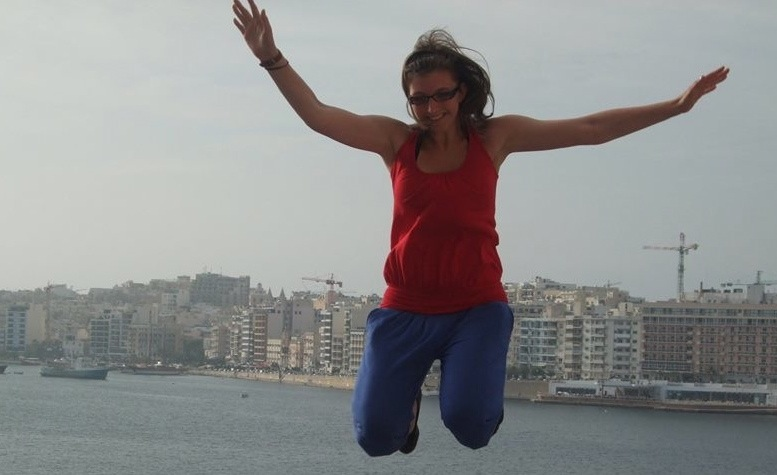
\includegraphics [scale=.30, angle=0]{Bild3.jpg}\\
\vfill
\large \bf Alles im Leben kommt zu mir mit Freude, Leichtigkeit und Herrlichkeit!\textsuperscript{\textregistered}
\end{center}
\end{figure}

\vfill
\vspace*{7mm}
\begin{center}
{\Huge \bf Lisa Marie Schack}\\
\vspace*{7mm}
Dillinger Straße 15\\
66793 Saarwellingen\\
Tel.: (0 68 38) 99 30 81\\
Mobil.: (0176) 79 40 44 14\\
\href{mailto:l.schacka@gmail.com}{l.schacka@gmail.com} \\
\end{center}

\vfill
\section{Zu meiner Person}
Lisa Marie Schack, wohnhaft in Saarwellingen, \\
Wassermann des Jahrgangs 1989.

\begin{tabular}{llp{50mm}l}
    Ausbildung: & \textbullet & Reiki 1995 \\
                & \textbullet & Reiki 2.Grad 2006 \\
                & \textbullet & Atlantis Lichtheilung 2011\\
                & \textbullet & Ayurvedische Gesichtsmassage März 2014\\
                & \textbullet & Acces Bars Facilitator August 2014\\
                & \textbullet & Masseurin für Kopfschmerzmassage Oktober 2014\\
                & \textbullet & Metamorphose Behandlung Oktober 2014\\
\end{tabular}


\newpage
%%%%%%%%%%%%%%%%%%%%%%%%%%%%%%%%%%%%%%%%%%%%%%%%%%%%%%%%%%%%%%%%%%%%%'
\section{ACCESS CONSCIOUSNESS \textsuperscript{\textregistered}}

\begin{flushleft}
Menschen ermächtigen zu wissen, dass sie wissen.\\
\vspace*{4mm}
Alles im Leben kommt zu mir mit Freude, Leichtigkeit und Herrlichkeit!\textsuperscript{\textregistered}\\
\vspace*{4mm}
Wie kann es jetzt noch besser werden? \\
\vspace*{4mm}
Access Consciousness\textsuperscript{\textregistered} lädt dich dazu ein. \\
\vspace*{4mm}
Der Einstiegs-Kurs in Access Consciousness\textsuperscript{\textregistered} ist der Bars-Kurs. Wusstest du, dass sich auf deinem Kopf 32 Punkte befinden, für die, wenn sie sanft berührt werden, einfach alles auflösen was dich davon abhält zu empfangen? Diese Punkte enthalten alle Gedanken, Ideen, Überzeugungen, Emotionen und Überlegungen, die Du in all deinen Leben gesammelt hast. Hier ist die Gelegenheit all das los zu lassen!\\
\vspace*{4mm}
In jeder Bars Sitzung können zwischen fünf und zehntausend Begrenzungen gelöscht werden. Jeder Bars Punkt hat einen spezifischen Bereich, der durch Berührung diese Begrenzungen auflöst. Jeder Bereich den Du verändern willst kann hiermit verändert werden! Die Bars Sitzung ist unglaublich entspannend und pflegend.\\
\vspace*{4mm}
Die Bars hat tausenden von Leuten geholfen viele Aspekte ihres Lebens zu verändern, wie zum Beispiel die Bereiche Schlafen, Gesundheit und Gewicht, Geld, Sex und Beziehungen, Stress und noch viel mehr! Das Schlimmste was bei einer Bars Sitzung geschehen kann ist, dass es sich so anfühlt als hättest Du eine wunderbare Massage bekommen. Und das Beste was passieren kann, ist dass sich dein ganzes Leben mit totaler Leichtigkeit zu etwas Großartigem entwickelt.\\
\vspace*{4mm}
"Wenn Du etwas in deinem Leben ändern möchtest, erwarte nicht, dass diese Veränderung im Außen beginnt."\\
\end{flushleft}

%\vspace*{180mm}
\begin{center}
Nähere Infos unter:\\
{\url{http://www.url-der-Seite.de/}} \\
\end{center}



\end{document}
